
%%%%%%%%%%%%%%%%%% PREAMBULE %%%%%%%%%%%%%%%%%%

\documentclass[aspectratio=169,utf8]{beamer}
%\documentclass[aspectratio=169,handout]{beamer}

\usetheme{Boadilla}
%\usecolortheme{seahorse}
\usecolortheme[RGB={245,66,24}]{structure}
\useoutertheme{infolines}

% packages
\usepackage{amsfonts,amsmath,amssymb,amsthm}
\usepackage[utf8]{inputenc}
\usepackage[T1]{fontenc}
\usepackage{lmodern}

\usepackage[francais]{babel}
\usepackage{fancybox}
\usepackage{graphicx}

\usepackage{float}
\usepackage{xfrac}

%\usepackage[usenames, x11names]{xcolor}
\usepackage{tikz}
\usepackage{pgfplots}
\usepackage{datetime}



%-----  Package unités -----
\usepackage{siunitx}
\sisetup{locale = FR,detect-all,per-mode = symbol}

%\usepackage{mathptmx}
%\usepackage{fouriernc}
%\usepackage{newcent}
%\usepackage[mathcal,mathbf]{euler}

%\usepackage{palatino}
%\usepackage{newcent}
% \usepackage[mathcal,mathbf]{euler}



% \usepackage{hyperref}
% \hypersetup{colorlinks=true, linkcolor=blue, urlcolor=blue,
% pdftitle={Exo7 - Exercices de mathématiques}, pdfauthor={Exo7}}


%section
% \usepackage{sectsty}
% \allsectionsfont{\bf}
%\sectionfont{\color{Tomato3}\upshape\selectfont}
%\subsectionfont{\color{Tomato4}\upshape\selectfont}

%----- Ensembles : entiers, reels, complexes -----
\newcommand{\Nn}{\mathbb{N}} \newcommand{\N}{\mathbb{N}}
\newcommand{\Zz}{\mathbb{Z}} \newcommand{\Z}{\mathbb{Z}}
\newcommand{\Qq}{\mathbb{Q}} \newcommand{\Q}{\mathbb{Q}}
\newcommand{\Rr}{\mathbb{R}} \newcommand{\R}{\mathbb{R}}
\newcommand{\Cc}{\mathbb{C}} 
\newcommand{\Kk}{\mathbb{K}} \newcommand{\K}{\mathbb{K}}

%----- Modifications de symboles -----
\renewcommand{\epsilon}{\varepsilon}
\renewcommand{\Re}{\mathop{\text{Re}}\nolimits}
\renewcommand{\Im}{\mathop{\text{Im}}\nolimits}
%\newcommand{\llbracket}{\left[\kern-0.15em\left[}
%\newcommand{\rrbracket}{\right]\kern-0.15em\right]}

\renewcommand{\ge}{\geqslant}
\renewcommand{\geq}{\geqslant}
\renewcommand{\le}{\leqslant}
\renewcommand{\leq}{\leqslant}
\renewcommand{\epsilon}{\varepsilon}

%----- Fonctions usuelles -----
\newcommand{\ch}{\mathop{\text{ch}}\nolimits}
\newcommand{\sh}{\mathop{\text{sh}}\nolimits}
\renewcommand{\tanh}{\mathop{\text{th}}\nolimits}
\newcommand{\cotan}{\mathop{\text{cotan}}\nolimits}
\newcommand{\Arcsin}{\mathop{\text{arcsin}}\nolimits}
\newcommand{\Arccos}{\mathop{\text{arccos}}\nolimits}
\newcommand{\Arctan}{\mathop{\text{arctan}}\nolimits}
\newcommand{\Argsh}{\mathop{\text{argsh}}\nolimits}
\newcommand{\Argch}{\mathop{\text{argch}}\nolimits}
\newcommand{\Argth}{\mathop{\text{argth}}\nolimits}
\newcommand{\pgcd}{\mathop{\text{pgcd}}\nolimits} 


%----- Commandes divers ------
\newcommand{\ii}{\mathrm{i}}
\newcommand{\dd}{\text{d}}
\newcommand{\id}{\mathop{\text{id}}\nolimits}
\newcommand{\Ker}{\mathop{\text{Ker}}\nolimits}
\newcommand{\Card}{\mathop{\text{Card}}\nolimits}
\newcommand{\Vect}{\mathop{\text{Vect}}\nolimits}
\newcommand{\Mat}{\mathop{\text{Mat}}\nolimits}
\newcommand{\rg}{\mathop{\text{rg}}\nolimits}
\newcommand{\tr}{\mathop{\text{tr}}\nolimits}


%----- Structure des exercices ------

\newtheoremstyle{styleexo}% name
{2ex}% Space above
{3ex}% Space below
{}% Body font
{}% Indent amount 1
{\bfseries} % Theorem head font
{}% Punctuation after theorem head
{\newline}% Space after theorem head 2
{}% Theorem head spec (can be left empty, meaning ‘normal’)

%\theoremstyle{styleexo}
\newtheorem{exo}{Exercice}
\newtheorem{ind}{Indications}
\newtheorem{cor}{Correction}


\newcommand{\exercice}[1]{} \newcommand{\finexercice}{}
%\newcommand{\exercice}[1]{{\tiny\texttt{#1}}\vspace{-2ex}} % pour afficher le numero absolu, l'auteur...
\newcommand{\enonce}{\begin{exo}} \newcommand{\finenonce}{\end{exo}}
\newcommand{\indication}{\begin{ind}} \newcommand{\finindication}{\end{ind}}
\newcommand{\correction}{\begin{cor}} \newcommand{\fincorrection}{\end{cor}}

\newcommand{\noindication}{\stepcounter{ind}}
\newcommand{\nocorrection}{\stepcounter{cor}}

\newcommand{\fiche}[1]{} \newcommand{\finfiche}{}
\newcommand{\titre}[1]{\centerline{\large \bf #1}}
\newcommand{\addcommand}[1]{}
\newcommand{\video}[1]{}

% Marge
\newcommand{\mymargin}[1]{\marginpar{{\small #1}}}

\def\noqed{\renewcommand{\qedsymbol}{}}


%----- Presentation ------
\setlength{\parindent}{0cm}

%\newcommand{\ExoSept}{\href{http://exo7.emath.fr}{\textbf{\textsf{Exo7}}}}

\definecolor{myred}{rgb}{0.93,0.26,0}
\definecolor{myorange}{rgb}{0.97,0.58,0}
\definecolor{myyellow}{rgb}{1,0.86,0}

\newcommand{\LogoExoSept}[1]{  % input : echelle
{\usefont{U}{cmss}{bx}{n}
\begin{tikzpicture}[scale=0.1*#1,transform shape]
  \fill[color=myorange] (0,0)--(4,0)--(4,-4)--(0,-4)--cycle;
  \fill[color=myred] (0,0)--(0,3)--(-3,3)--(-3,0)--cycle;
  \fill[color=myyellow] (4,0)--(7,4)--(3,7)--(0,3)--cycle;
  \node[scale=5] at (3.5,3.5) {Exo7};
\end{tikzpicture}}
}


\newcommand{\debutmontitre}{
  \author{} \date{} 
  \thispagestyle{empty}
  \hspace*{-10ex}
  \begin{minipage}{\textwidth}
    \titlepage  
  \vspace*{-2.5cm}
  \begin{center}
    \LogoExoSept{2.5}
  \end{center}
  \end{minipage}

  \vspace*{-0cm}
  
  % Astuce pour que le background ne soit pas discrétisé lors de la conversion pdf -> png
\begin{tikzpicture}
        \fill[opacity=0,green!60!black] (0,0)--++(0,0)--++(0,0)--++(0,0)--cycle; 
\end{tikzpicture}

% toc S'affiche trop tot :
% \tableofcontents[hideallsubsections, pausesections]
}

\newcommand{\finmontitre}{
  \end{frame}
  \setcounter{framenumber}{0}
} % ne marche pas pour une raison obscure

%----- Commandes supplementaires ------

% \usepackage[landscape]{geometry}
% \geometry{top=1cm, bottom=3cm, left=2cm, right=10cm, marginparsep=1cm
% }
% \usepackage[a4paper]{geometry}
% \geometry{top=2cm, bottom=2cm, left=2cm, right=2cm, marginparsep=1cm
% }

%\usepackage{standalone}


% New command Arnaud -- november 2011
\setbeamersize{text margin left=24ex}
% si vous modifier cette valeur il faut aussi
% modifier le decalage du titre pour compenser
% (ex : ici =+10ex, titre =-5ex

\theoremstyle{definition}
%\newtheorem{proposition}{Proposition}
%\newtheorem{exemple}{Exemple}
%\newtheorem{theoreme}{Théorème}
%\newtheorem{lemme}{Lemme}
%\newtheorem{corollaire}{Corollaire}
%\newtheorem*{remarque*}{Remarque}
%\newtheorem*{miniexercice}{Mini-exercices}
%\newtheorem{definition}{Définition}

% Commande tikz
\usetikzlibrary{calc}
\usetikzlibrary{patterns,arrows}
\usetikzlibrary{matrix}
\usetikzlibrary{fadings} 

%definition d'un terme
\newcommand{\defi}[1]{{\color{myorange}\textbf{\emph{#1}}}}
\newcommand{\evidence}[1]{{\color{blue}\textbf{\emph{#1}}}}
\newcommand{\assertion}[1]{\emph{\og#1\fg}}  % pour chapitre logique
%\renewcommand{\contentsname}{Sommaire}
\renewcommand{\contentsname}{}
\setcounter{tocdepth}{2}



%------ Figures ------

\def\myscale{1} % par défaut 
\newcommand{\myfigure}[2]{  % entrée : echelle, fichier figure
\def\myscale{#1}
\begin{center}
\footnotesize
{#2}
\end{center}}


%------ Encadrement ------

\usepackage{fancybox}


\newcommand{\mybox}[1]{
\setlength{\fboxsep}{7pt}
\begin{center}
\shadowbox{#1}
\end{center}}

\newcommand{\myboxinline}[1]{
\setlength{\fboxsep}{5pt}
\raisebox{-10pt}{
\shadowbox{#1}
}
}

%--------------- Commande beamer---------------
\newcommand{\beameronly}[1]{#1} % permet de mettre des pause dans beamer pas dans poly


\setbeamertemplate{navigation symbols}{}
\setbeamertemplate{footline}  % tiré du fichier beamerouterinfolines.sty
{
  \leavevmode%
  \hbox{%
  \begin{beamercolorbox}[wd=.333333\paperwidth,ht=2.25ex,dp=1ex,center]{author in head/foot}%
    % \usebeamerfont{author in head/foot}\insertshortauthor%~~(\insertshortinstitute)
    \usebeamerfont{section in head/foot}{\bf\insertshorttitle}
  \end{beamercolorbox}%
  \begin{beamercolorbox}[wd=.333333\paperwidth,ht=2.25ex,dp=1ex,center]{title in head/foot}%
    \usebeamerfont{section in head/foot}{\bf\insertsectionhead}
  \end{beamercolorbox}%
  \begin{beamercolorbox}[wd=.333333\paperwidth,ht=2.25ex,dp=1ex,right]{date in head/foot}%
    % \usebeamerfont{date in head/foot}\insertshortdate{}\hspace*{2em}
    \insertframenumber{} / \inserttotalframenumber\hspace*{2ex} 
  \end{beamercolorbox}}%
  \vskip0pt%
}


\definecolor{mygrey}{rgb}{0.5,0.5,0.5}
\setlength{\parindent}{0cm}
%\DeclareTextFontCommand{\helvetica}{\fontfamily{phv}\selectfont}

% background beamer
\definecolor{couleurhaut}{rgb}{0.85,0.9,1}  % creme
\definecolor{couleurmilieu}{rgb}{1,1,1}  % vert pale
\definecolor{couleurbas}{rgb}{0.85,0.9,1}  % blanc
\setbeamertemplate{background canvas}[vertical shading]%
[top=couleurhaut,middle=couleurmilieu,midpoint=0.4,bottom=couleurbas] 
%[top=fondtitre!05,bottom=fondtitre!60]



\makeatletter
\setbeamertemplate{theorem begin}
{%
  \begin{\inserttheoremblockenv}
  {%
    \inserttheoremheadfont
    \inserttheoremname
    \inserttheoremnumber
    \ifx\inserttheoremaddition\@empty\else\ (\inserttheoremaddition)\fi%
    \inserttheorempunctuation
  }%
}
\setbeamertemplate{theorem end}{\end{\inserttheoremblockenv}}

\newenvironment{theoreme}[1][]{%
   \setbeamercolor{block title}{fg=structure,bg=structure!40}
   \setbeamercolor{block body}{fg=black,bg=structure!10}
   \begin{block}{{\bf Th\'eor\`eme }#1}
}{%
   \end{block}%
}


\newenvironment{proposition}[1][]{%
   \setbeamercolor{block title}{fg=structure,bg=structure!40}
   \setbeamercolor{block body}{fg=black,bg=structure!10}
   \begin{block}{{\bf Proposition }#1}
}{%
   \end{block}%
}

\newenvironment{corollaire}[1][]{%
   \setbeamercolor{block title}{fg=structure,bg=structure!40}
   \setbeamercolor{block body}{fg=black,bg=structure!10}
   \begin{block}{{\bf Corollaire }#1}
}{%
   \end{block}%
}

\newenvironment{mydefinition}[1][]{%
   \setbeamercolor{block title}{fg=structure,bg=structure!40}
   \setbeamercolor{block body}{fg=black,bg=structure!10}
   \begin{block}{{\bf Définition} #1}
}{%
   \end{block}%
}

\newenvironment{lemme}[0]{%
   \setbeamercolor{block title}{fg=structure,bg=structure!40}
   \setbeamercolor{block body}{fg=black,bg=structure!10}
   \begin{block}{\bf Lemme}
}{%
   \end{block}%
}

\newenvironment{remarque}[1][]{%
   \setbeamercolor{block title}{fg=black,bg=structure!20}
   \setbeamercolor{block body}{fg=black,bg=structure!5}
   \begin{block}{Remarque #1}
}{%
   \end{block}%
}


\newenvironment{exemple}[1][]{%
   \setbeamercolor{block title}{fg=black,bg=structure!20}
   \setbeamercolor{block body}{fg=black,bg=structure!5}
   \begin{block}{{\bf Exemple }#1}
}{%
   \end{block}%
}


\newenvironment{miniexercice}[0]{%
   \setbeamercolor{block title}{fg=structure,bg=structure!20}
   \setbeamercolor{block body}{fg=black,bg=structure!5}
   \begin{block}{Mini-exercices}
}{%
   \end{block}%
}


\newenvironment{tp}[0]{%
   \setbeamercolor{block title}{fg=structure,bg=structure!40}
   \setbeamercolor{block body}{fg=black,bg=structure!10}
   \begin{block}{\bf Travaux pratiques}
}{%
   \end{block}%
}
\newenvironment{exercicecours}[1][]{%
   \setbeamercolor{block title}{fg=structure,bg=structure!40}
   \setbeamercolor{block body}{fg=black,bg=structure!10}
   \begin{block}{{\bf Exercice }#1}
}{%
   \end{block}%
}
\newenvironment{algo}[1][]{%
   \setbeamercolor{block title}{fg=structure,bg=structure!40}
   \setbeamercolor{block body}{fg=black,bg=structure!10}
   \begin{block}{{\bf Algorithme}\hfill{\color{gray}\texttt{#1}}}
}{%
   \end{block}%
}


\setbeamertemplate{proof begin}{
   \setbeamercolor{block title}{fg=black,bg=structure!20}
   \setbeamercolor{block body}{fg=black,bg=structure!5}
   \begin{block}{{\footnotesize Démonstration}}
   \footnotesize
   \smallskip}
\setbeamertemplate{proof end}{%
   \end{block}}
\setbeamertemplate{qed symbol}{\openbox}


\makeatother
\usecolortheme[RGB={127,0,0}]{structure}

% Commande spécifique à ce chapitre

\newcommand{\Python}{\texttt{Python}}
\renewcommand{\evidence}[1]{{\color{blue}\textbf{#1}}}

\usepackage{textcomp}

\usepackage{listings}
\lstset{
  upquote=true,
  columns=flexible,
  keepspaces=true,
  basicstyle=\ttfamily,
  commentstyle=\color{gray},
  language=Python,
  showstringspaces=false,
  aboveskip=0em,  
  belowskip=0em,
  escapeinside=||
}

\lstset{
  literate={é}{{\'e}}1
           {è}{{\`e}}1
           {à}{{\`a}}1
}


\newcommand{\codeinline}[1]{\lstinline!#1!}

\definecolor{coul_prive}{rgb}{0.93,0.26,0}
\definecolor{coul_public}{rgb}{0.06,0.63,0}

\newcommand{\prive}[1]{{\bf\color{coul_prive} #1}}
\newcommand{\public}[1]{{\bf\color{coul_public} #1}}

%%%%%%%%%%%%%%%%%%%%%%%%%%%%%%%%%%%%%%%%%%%%%%%%%%%%%%%%%%%%%
%%%%%%%%%%%%%%%%%%%%%%%%%%%%%%%%%%%%%%%%%%%%%%%%%%%%%%%%%%%%%


\begin{document}


\title{{\bf Cryptographie}}
\subtitle{La cryptographie à clé publique}

\begin{frame}
  
  \debutmontitre

  \pause

{\footnotesize
\hfill
\setbeamercovered{transparent=50}
\begin{minipage}{0.6\textwidth}
  \begin{itemize}
    \item<3-> Le principe de Kerckhoffs
    \item<4-> Factorisation des entiers
    \item<5-> Fonctions à sens unique
    \item<6-> Chiffrement à clé privée
    \item<7-> Chiffrement à clé publique
  \end{itemize}
\end{minipage}
}

\end{frame}

\setcounter{framenumber}{0}


%%%%%%%%%%%%%%%%%%%%%%%%%%%%%%%%%%%%%%%%%%%%%%%%%%%%%%%%%%%%%%%%
\section{Le principe de Kerckhoffs}

\begin{frame}


\evidence{Principe de Kerckhoffs}

\pause

\mybox{
\begin{minipage}{0.6\textwidth}
\sl\centering La sécurité d'un système de chiffrement
ne doit reposer que sur le secret de la clé. 
\end{minipage}
}

\pause

\mybox{\sl L'ennemi peut avoir connaissance du système de chiffrement.}

\pause

\begin{itemize}
  \item Contraire à l'intuition qui est de dissimuler le maximum de choses possibles
\pause
  \item Un mécanisme connu de tous sera testé, attaqué, étudié, 
et utilisé s'il est robuste
\pause
  \item Seule la clé utilisée reste secrète
  
\end{itemize}

\end{frame}



%%%%%%%%%%%%%%%%%%%%%%%%%%%%%%%%%%%%%%%%%%%%%%%%%%%%%%%%%%%%%%%%
\section{Factorisations des entiers}

\begin{frame}

\evidence{Complexité de la factorisation}

\pause
\begin{itemize}
  \item $5\times7 = ?$
  \pause
  \item $35 = ?$
  \pause
  \item Factoriser $1591$
  \pause
  \item Calculer $37\times 43$
  \pause
  \item Calculer $p \times q$ est plus facile que de factoriser $n=pq$
\end{itemize}

\bigskip
\pause

\begin{itemize}
  \item La \defi{complexité} estime le temps de calcul (ou le nombre d'opérations élémentaires)
  nécessaire pour effectuer une opération
  \pause
  
  \item \evidence{Addition}
  \begin{itemize}
  \pause
    \item La somme de deux chiffres (par exemple $6+8$) est de complexité $1$
    \pause
    \item La somme de deux entiers à $n$ chiffres est de complexité $n$
    \pause
    \item Ex. $1234+2323$ : $4$ additions de chiffres
   \end{itemize}
  
  \pause
  \item \evidence{Multiplication}
  \pause
  \begin{itemize}
    \item La multiplication de deux entiers à $n$ chiffres est de complexité $n^2$
    \pause
    \item Ex. $1234 \times 2323$ : $16$ multiplications de chiffres
   \end{itemize}
   
  \pause 
  \item \evidence{Factorisation} : $\exp(4n^\frac13)$
   
\end{itemize}
\end{frame}


\begin{frame}

\evidence{Multiplier et factoriser des nombres à $n$ chiffres}
\begin{center}
\begin{tabular}{ccc}

$n$ & multiplication & factorisation \\
\hline
3 & 9 & 320 \\
4 & 16 & 572 \\
5 & 25 & 934 \\
10 & 100 & 5\;528 \\
50 & 2\;500 & 2\;510\;835 \\
100 & 10\;000 & 115\;681\;968 \\
200 & 40\;000 & 14\;423\;748\;780 \\
\end{tabular}  
\end{center}
\end{frame}


%%%%%%%%%%%%%%%%%%%%%%%%%%%%%%%%%%%%%%%%%%%%%%%%%%%%%%%%%%%%%%%%
\section{Fonctions à sens unique}

\begin{frame}

\evidence{Fonctions à sens unique}
\pause
\begin{itemize}
  \item Fonction $f$
  \pause
  \item Connaissant $x$, calcul <<facile>> de $f(x)$
  \pause
  \item Pour un $y$, trouver $x$ tel que $y=f(x)$ est <<difficile>>
  \pause
  \item Fonction à sens unique à \defi{trappe}
\end{itemize}

\bigskip
\pause
\bigskip

Exemple : 
$$f : x\longmapsto x^3 \pmod{100}$$

Trouver $x$ tel que $x^3 \equiv 11 \pmod{100}$
\pause

  \begin{itemize}
  \item Recherche exhaustive, tester $0$, $1$, $2$, $3$, ...,  $99$
  \pause
    $$
    71^3=357\;911 \equiv 11 \pmod{100}
    $$
    
  \pause  
  \item Trappe secrète : $y \longmapsto y^7 \pmod{100}$ qui 
  fournit directement le résultat !
  \pause
    $$
    11^7= 19\;487\;171 \equiv 71 \pmod{100}
    $$
  \end{itemize}

\end{frame}


%%%%%%%%%%%%%%%%%%%%%%%%%%%%%%%%%%%%%%%%%%%%%%%%%%%%%%%%%%%%%%%%
\section{Chiffrement à clé privée}

\begin{frame}

\evidence{Chiffrement à clé privée}

\bigskip\bigskip

\begin{center}
\hspace*{-10mm}
\begin{tikzpicture}[scale=0.8]

  \node at (4,3) {\bf ALICE};
  \node at (-4,3) {\bf BRUNO};
  
  \draw[line width=5pt,>=stealth,->,gray] (-2.1,0) to (2.1,0);
  
  \node at (-6,1.7) {\prive{Message M}};
  \node at (6,1.7) {\prive{Message M}};
  \node at (-0.05,0.5) {\public{Message crypté X}};  
  \node at (0,1.9) {\bf \prive{Clé C}};  
  \draw (-4,0)node[draw]{Chiffrement  \public{$\mathcal{C}$}};
  \draw (4.2,0)node[draw]{Déchiffrement  \public{$\mathcal{D}$}};
  
  \draw[->, blue, very thick] (-0.7,1.8) to[bend right, thick] (-3.2,0.5);
  \draw[->, blue, very thick] (0.7,1.8) to[bend left, thick] (3.2,0.5);
 
  \draw[->, blue, very thick] (-5,1.5) to (-4.5,0.5);
  \draw[<-, blue, very thick] (5,1.5) to (4.5,0.5);
\end{tikzpicture}  
\end{center}
\end{frame}

\begin{frame}

\evidence{Chiffrement à clé privée}

\bigskip

\begin{center}
\begin{tikzpicture}[scale=0.9]
  \node at (-0.50,0){
  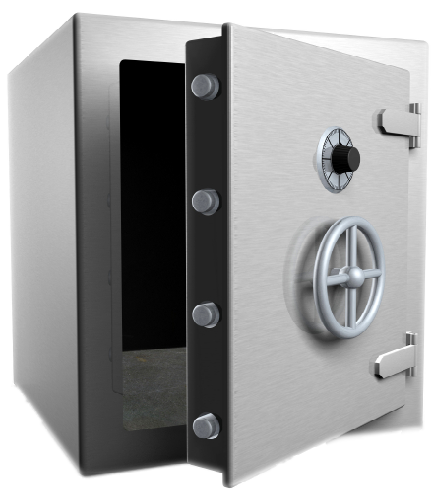
\includegraphics[height=4.5cm]{figures/coffre.png}
  };
  \node at (-3,-3) {\bf ALICE};
  \node at (-5,-1) {\bf BRUNO};
  
  \draw[->, blue, ultra thick] (-5,-0.7) to[bend left, thick]node[above, midway]{} (-1,0);
  \draw[->, blue, ultra thick] (-1.2,-0.5) to[bend right, thick]node[above, midway]{} (-3,-2.7);

\end{tikzpicture}  
\end{center}
\end{frame}


%%%%%%%%%%%%%%%%%%%%%%%%%%%%%%%%%%%%%%%%%%%%%%%%%%%%%%%%%%%%%%%%
\section{Chiffrement à clé publique}

\begin{frame}

\evidence{Chiffrement à clé publique}

\bigskip

\begin{center}
\begin{tikzpicture}
  \node at (+0.6,-0.56){
  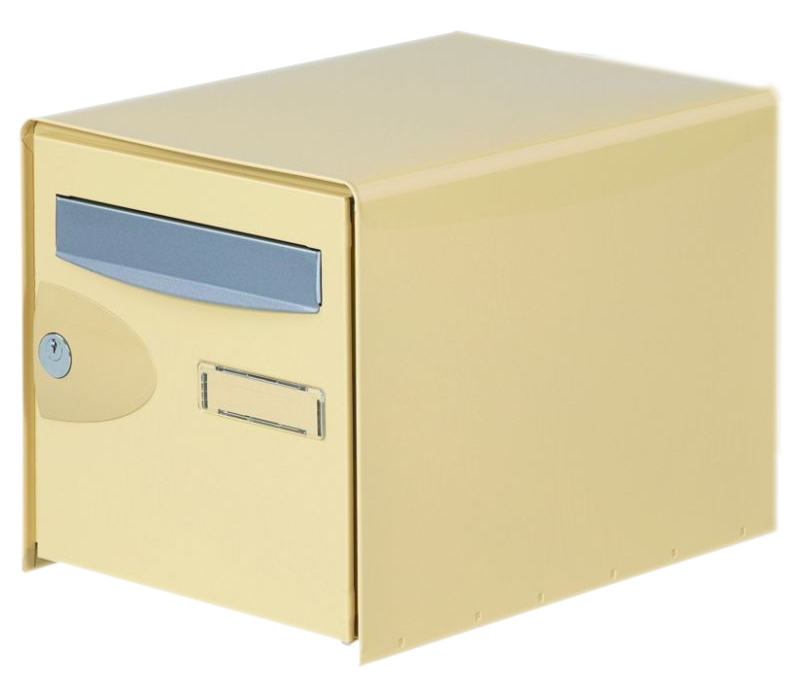
\includegraphics[height=5cm]{figures/boite.png}
  };
  \node at (-3,-3) {\bf ALICE};
  \node at (-5,-1) {\bf BRUNO};
  
  \draw[->, myred, ultra thick] (-5,-0.7) to[bend left, thick]node[above, midway]{} (-1,0);
  \draw[->, myred, ultra thick] (-2.,-0.7) to[bend right, thick]node[above, midway]{} (-3,-2.7);

\end{tikzpicture}  
\end{center}
\end{frame}


\begin{frame}

\evidence{Chiffrement à clé publique}

\bigskip\bigskip

\begin{center}
\hspace*{-10mm}
\begin{tikzpicture}[scale=0.8]

  \node at (4,3) {\bf ALICE};
  \node at (-4,3) {\bf BRUNO};
  
  \draw[line width=5pt,>=stealth,->,gray] (-2.1,0) to (2.1,0);
  
  \node at (-6,1.7) {\prive{Message M}};
  \node at (6,1.7) {\prive{Message M}};
  \node at (0,0.5) {\public{Message crypté X}};  
  \node at (2.5,2.3) {\bf \public{Clé publique}};  
  \node at (2.5,1.7) {\bf \prive{Clé privée}}; 
  \draw (-4,0)node[draw]{Chiffrement  \public{$\mathcal{C}$}};
  \draw (4.2,0)node[draw]{Déchiffrement \public{$\mathcal{D}$}};
  
  \draw[->, blue, very thick] (1.1,2.3) to[bend right, thick] (-3.2,0.5);
  \draw[->, blue, very thick] (2.8,1.5) to[bend left, thick] (3.5,0.5);
 
  \draw[->, blue, very thick] (-5,1.5) to (-4.5,0.5);
  \draw[<-, blue, very thick] (5,1.5) to (4.5,0.5);
\end{tikzpicture}  
\end{center}
\end{frame}


\begin{frame}
Paramètres d'un \defi{chiffrement à clé publique}
\pause
\begin{enumerate}
\item les fonctions de chiffrement et de déchiffrement \public{$\mathcal{C}$} et \public{$\mathcal{D}$}
\pause
\item la clé publique du destinataire qui paramètre la fonction \public{$\mathcal{C}$}
\pause
\item la clé privée du destinataire qui paramètre la fonction \public{$\mathcal{D}$}
\end{enumerate}

\bigskip
\pause 
\begin{center}
Trouver $x$ tel que $x^3 \equiv 11 \pmod{100}$
\end{center}
\bigskip
\pause

\begin{enumerate}
\item \public{$\mathcal{C}$} : $x\longmapsto x^\text{\bf ?} \pmod{100}$ et \public{$\mathcal{D}$} : $x\longmapsto x^\text{\bf ?} \pmod{100}$
\pause
\item la clé publique d'Alice \public{3}  \quad $\public{\mathcal{C}} : x\longmapsto x^\public{3} \pmod{100}$
\pause
\item la clé privée d'Alice \prive{7}  \quad $\prive{\mathcal{D}} : x\longmapsto x^\prive{7} \pmod{100}$ 
\end{enumerate}
\end{frame}


\end{document}
